% =========================================================================
% NeurIPS 2026 Workshop "Who Verifies the Agents?" (Verify-Agents) submission
% Verification-framed workshop cut of the STJP paper.
% Build: pdflatex -> bibtex -> pdflatex x2  (see Makefile)
% Anonymous, double-blind. 4-9 pages main text excl. references/appendix.
% =========================================================================
\documentclass{article}
\usepackage[]{neurips_2026}      % submission (anonymous) mode; add [final] for camera-ready
\usepackage[utf8]{inputenc}
\usepackage[T1]{fontenc}
\usepackage{amsmath,amssymb}
\usepackage{graphicx}
\usepackage{booktabs}
\usepackage{multirow}
\usepackage{xcolor}
\usepackage{microtype}
\usepackage{url}
\usepackage{hyperref}
\hypersetup{colorlinks=true,linkcolor=blue!55!black,citecolor=blue!55!black,urlcolor=blue!55!black}

% Workshop notice line (double-blind submission)
\makeatletter
\renewcommand{\@noticestring}{Submitted to the NeurIPS 2026 Workshop ``Who Verifies the Agents? Toward Reliable Agent Development.'' Do not distribute.}
\makeatother

% notation macros
\newcommand{\gtG}{\mathsf{G}}
\newcommand{\proj}[2]{#1\!\upharpoonright\!#2}
\newcommand{\stjp}{\textsc{STJP}}

\title{The Compiler Verifies the Agents:\\ Session-Typed Static and Runtime Verification\\ for Multi-Agent LLM Coordination}

\author{%
  Anonymous Author(s)\\
}

\begin{document}
\maketitle

\begin{abstract}
To verify an agent one must first fix a basis to verify it against---the oracle problem of software testing, which for LLM agents takes the form of a specification, a skill file, or an agent markdown. Existing instruments only check behavior against that basis. Runs exhibit single executions and LLM judges of contested reliability score traces; neither certifies the absence of failure. No system asks whether the basis itself is sound and complete as a coordination discipline, free of deadlock and able to reach its goal, so errors that are decidable statically surface only after runtime resources have been spent. We present \stjp{}, a compiler-verifier for multi-agent coordination grounded in multiparty session types. An LLM drafts the user's intent as a Scribble global protocol; a static checker verifies it before any agent runs; and the validated type is projected into per-role contracts, deterministic monitors, guards, and a scheduler that enforce it on free-running, untrusted agents at the message boundary. Every metric is computed mechanically over a typed event log, without golden trajectories or LLM judges. The verifiers are themselves verified. Mutation testing detects 95.1\% of seeded defects with zero false positives, the gate with value refinements blocks all 1{,}200 red-team exfiltration attempts, and we audit the fairness of our own harness. At $n{=}100$, unenforced protocol text reaches the goal in 100 of 100 trials while committing a forbidden irreversible act in 95 of them, whereas every enforcing arm shows zero disasters at every model tier and the full stack is also the cheapest, by $4$--$22\times$ on cost to clean goal. A seeded circular-wait deadlock is rejected statically at zero token cost. Testing observes runs; typing quantifies over all of them.
\end{abstract}

\section{Introduction}\label{sec:intro}
Verification presupposes a basis to verify against. In program verification that basis is the assertion of Hoare logic \citep{hoare69}; in software testing it is the oracle, and the impossibility of judging observed behavior without one is the classical oracle problem \citep{barr15}. For LLM agents the basis is today a specification, a policy, or a skill file, and the instruments that consult it are both downstream of execution. Benchmarks and trace evaluators measure, after the fact, how often agents violated policy \citep{stweb,besafe}, while LLM-as-judge pipelines score transcripts with a second model whose own reliability is contested---reported true-negative rates fall below 25\% and expert agreement reaches only 64--68\% \citep{judgebias}---and whose scores invite exactly the reward hacking this workshop names. Both observe executions against a verification basis, a spec or policy or skill file, whose own soundness nothing checks. No instrument asks whether the artifact the agents will faithfully follow can deadlock them, strand them short of the goal, or leave a role's duties hanging on a choice it cannot observe. Neither can certify a specification, and testing, as Dijkstra observed, shows the presence of bugs, never their absence \citep{dijkstra72}.

The gap matters most where agents meet each other. The largest empirical study of multi-agent failures, MAST, annotated 1{,}600+ traces across seven frameworks and found failures clustering not in model weakness but in \emph{system design issues, inter-agent misalignment, and task verification} \citep{mast}. The artifacts that fix this interaction discipline---\texttt{SKILL.md} files, \texttt{AGENTS.md} conventions, MCP manifests, enterprise agent specs \citep{anthropic-skills}---are, functionally, programs. They say which role sends which message to which role, in what order, with which authorization preceding which irreversible act. Yet no tool verifies them. Format linting exists, and 34\% of community skill packages violate even the published format spec \citep{skilldex}, but format validity says nothing about interaction soundness. A skill can parse perfectly while describing a choreography in which the planner waits for a result the worker will never send, because the worker is waiting for an answer the planner cannot give. Nothing crashes; the system sits there, emitting tokens.

This paper answers the workshop's question in its static form. \textbf{The verifier is a compiler, and it runs before any agent does.} \stjp{} (Session-Typed skills/Judge Protocol) is a pipeline built on multiparty session type theory \citep{hyc08,scalas19} and its protocol language Scribble \citep{scribble}. The user states an intent; an LLM drafts a Scribble global protocol; the checker verifies well-formedness statically---rejecting deadlock precursors, incoherent choice, unguarded recursion, unreachable goals---and only a validated protocol is projected, role by role, into local contracts that become each agent's lean skill. From the same projection we mechanically generate a deterministic finite-state monitor per role, value-dependent choice guards in the asserted-MPST style \citep{bocchi10}, and a scheduler. The LLM-drafted protocol is an \emph{agent-generated artifact under formal verification}; the agents stay free-running and untrusted, and the monitorability theorem \citep{bocchi13} guarantees that local $O(1)$ boundary checks compose to global compliance---in contrast to concurrent work that obtains guarantees by generating the coordination layer as trusted code around opaque LLM calls \citep{bollig26}.

Three properties make this a verification-workshop contribution rather than only a systems one.

\textbf{(1) The verification signal is deterministic and judge-free.} Because every run is, by construction, a path through a validated global type, conformance and goal achievement receive mechanical, bit-reproducible definitions over a typed event log, with no hand-authored golden trajectory and no LLM judge (\S\ref{sec:method}). The judged surface shrinks to what is genuinely semantic; a verifier that is plain code cannot be sweet-talked, and there is no scalar reward to game.

\textbf{(2) The verifiers are themselves verified---including against us.} We mutation-test the static checker against 626 seeded defects (95.1\% well-formedness detection, zero false positives, one named residual gap), red-team the runtime gate with 1{,}200 injected exfiltration attempts (91.7\%; with value refinements, 100\%), hand-derive a 40-trace verdict corpus for monitor and grader, forensically audit all 1{,}200 benchmark trials, and---after asking \emph{did we rig the grading?}---publish a fairness audit of our own harness that found five ways it had favored our system (\S\ref{sec:verify}).

\textbf{(3) Verification stays faithful as agents evolve.} A measured capability sweep across three Claude tiers shows that unenforced safety is capability-\emph{dependent}, with premature irreversible filings going 95$\to$0$\to$0 on identical protocol text, while the enforcing arm remains capability-\emph{invariant} at 100\% clean-goal completion and zero disasters at every tier (\S\ref{sec:findings}). The closing gap is an average; the gate's zero is a guarantee.

These contributions map directly onto the workshop's pillars---robust, ungameable verifiers and red-teamed evaluation harnesses; runtime verification and benchmarks that stress-test the verification method itself; heterogeneous signals beyond scalar reward; formal verification of an agent-generated artifact; and Agent4Agent verification, since the drafter is an agent whose output governs other agents.

\section{Related work}\label{sec:related}
\textbf{Governance layers and runtime enforcement.} Recent syntheses organize agent governance as a three-layer stack \citep{governspec,lga}. Layer~0 checks that a specification parses and is commoditized \citep{skilldex}; Layer~2 measures whether runtime behavior matches claims and is an active benchmark frontier \citep{besafe,stweb}; Layer~1, which asks whether the specification is semantically sound, is in those surveys' words ``not available.'' \stjp{} occupies it. Runtime guardrails act per execution. AgentSpec \citep{agentspec} enforces trigger/predicate/action rules around tool calls, Agent-C \citep{agentc} compiles temporal constraints to SMT checks, and LGA \citep{lga} composes sandboxing and audit logging. Rule DSLs cannot express, let alone verify, \emph{global} interaction properties---deadlock-freedom, goal reachability, choice coherence---because these are properties of the protocol structure, not of any single call. \stjp{} rejects the faulty specification before the first LLM call, the only point at which a guarantee can be universal rather than per-run; its runtime gate then enforces exactly the properties the static phase proved enforceable \citep{bocchi13}. We are explicit about where the novelty lies. The session-type theory is three decades deep and is assembled here, not invented; our contributions are the compiler-verifier framing, the gradual-typing integration of an untyped LLM participant \citep{igarashi17}, the observation that the scheduler is itself a projection artifact, and the judge-free empirical program this paper executes.

\textbf{Projection-based coordination for LLM agents.} Concurrently, \citet{bollig26} introduce an MSC-based DSL (ZipperGen) whose projection yields deadlock-free local programs by construction, machine-checked in Lean~4---a mechanization discipline we do not match and admire. The systems are separated by the trust boundary. In ZipperGen the LLM never holds the send keys, since coordination is trusted generated code---a clean closed-world result that cannot govern the deployed ecosystem, where free-running agents \emph{are} the message-senders. \stjp{} targets that open regime, in which the LLM is the untyped participant of gradual session types, the monitor is the cast at the boundary, and the operative theorem is monitorability; every phenomenon we measure exists only there, and \citet{bollig26} report no empirical evaluation. Certified MPST projection \citep{listutz23,liwies25} is our named upgrade path; trace-based assurance \citep{paduraru26} is downstream of the static question posed here.

\textbf{Trace evaluation.} Tool-and-step, process-utility \citep{trace}, policy-conditioned \citep{stweb}, and reliability ($\mathrm{pass}^k$) metrics all presuppose a hand-authored reference trajectory or an LLM judge, because an unconstrained agent leaves no structure to score a run against. Under \stjp{}, the validated global type \emph{is} the reference.

\begin{table}[t]
\centering\small
\caption{Positioning. \stjp{} is, to our knowledge, the only system that both establishes guarantees \emph{before} execution and enforces them on \emph{untrusted} agents at runtime, with evaluation requiring neither a reference trajectory nor an LLM judge. ``partial'' = expressible per hand-written rule, without a global theorem. ``n/a$^{\dagger}$'' marks that in \citet{bollig26} agents cannot address messages at all, so recipient legality is moot rather than checked.}
\label{tab:position}
\resizebox{\textwidth}{!}{\begin{tabular}{@{}lcccccc@{}}
\toprule
& \textbf{When it acts} & \textbf{Deadlock-} & \textbf{Goal reach-} & \textbf{Unauth.\ recip.} & \textbf{Value/branch} & \textbf{Judge-free} \\
& & \textbf{freedom} & \textbf{ability} & \textbf{blocked} & \textbf{guards} & \textbf{metrics} \\
\midrule
LLM-as-judge & post hoc & no & no & no & no & no \\
Rule guards \citep{agentspec} & runtime & no & no & partial & partial & no \\
Temporal/SMT \citep{agentc} & runtime & no & no & partial & partial & no \\
Graph frameworks & wiring & no & no & no & no & no \\
MSC codegen \citep{bollig26} & compile & static & no & n/a$^{\dagger}$ & no & no \\
\textbf{\stjp{} (this work)} & \textbf{compile $+$ runtime} & \textbf{static} & \textbf{static} & \textbf{typed} & \textbf{yes} & \textbf{yes} \\
\bottomrule
\end{tabular}}
\end{table}

\section{Verified properties, in sixty seconds}\label{sec:mpst}
A \emph{global type} $\gtG$ describes a whole conversation (roles, message labels, payload sorts, branching, guarded recursion); \emph{projection} $\proj{\gtG}{r}$ extracts role $r$'s local view, which induces a finite endpoint state machine (EFSM). A global type is \emph{well-formed} if it projects onto every role and recursion is guarded; the merge condition rejects protocols in which a role's duties silently depend on a decision it was never told about---already a useful lint. Four classical theorems then transfer \citep{hyc08,scalas19,bocchi13}. \textbf{T1 communication safety} guarantees that no role ever receives a message it cannot handle; \textbf{T2 session fidelity} guarantees that every execution trace refines $\gtG$; \textbf{T3 deadlock-freedom} guarantees that a well-typed single-session configuration never sticks; and \textbf{T4 monitorability} guarantees that if every endpoint is wrapped by a monitor enforcing its projected local type, the observable behavior of the whole \emph{untrusted} network satisfies $\gtG$, so local checks compose to a global guarantee with no central observer. T4 licenses the architecture---LLM endpoints stay untrusted, monitors are generated from projections, and global compliance falls out of local, $O(1)$-per-event checking. Asserted/refined MPST \citep{bocchi10,chen12} adds payload predicates and \emph{choice guards}, closing the ``protocol-legal but value-wrong'' hole (skipping the audit on \$50k$+$ revenue is legal for classical MPST, a violation for guarded MPST). Appendix~\ref{app:guar} tabulates the operational meaning of each guarantee.



\section{The \stjp{} verifier stack}\label{sec:system}
\begin{figure}[t]
\centering
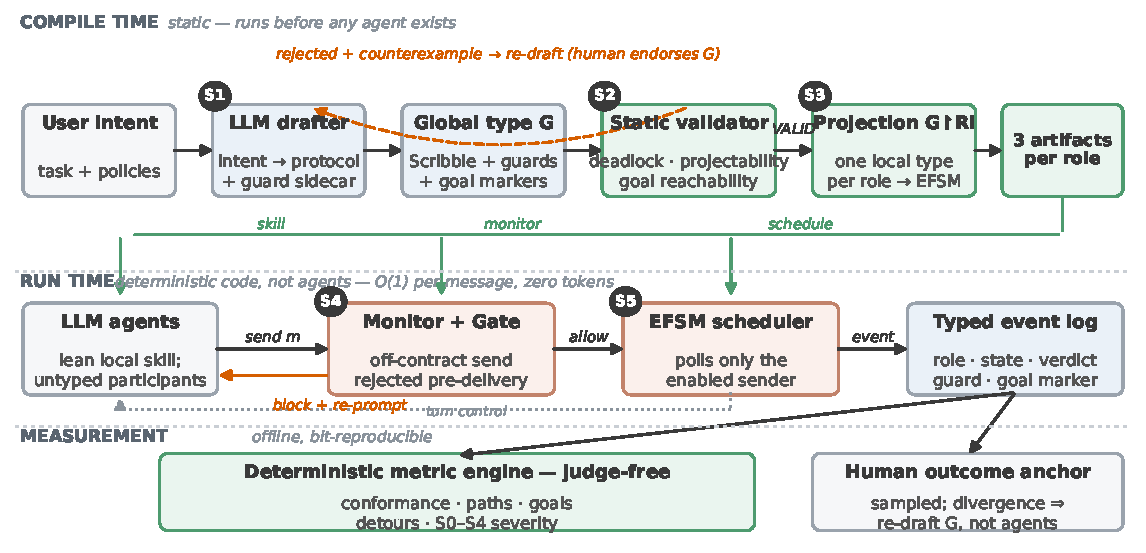
\includegraphics[width=\textwidth]{fig1_system.pdf}
\caption{\textbf{The \stjp{} pipeline.} At compile time an LLM drafts the user's intent as a Scribble global type with a guard sidecar; the static validator rejects unsafe drafts with counterexamples, and only a validated $\gtG$ is projected into three artifacts per role---a lean local contract, a generated EFSM monitor, and the schedule. At run time the gate rejects off-contract sends \emph{pre-delivery} and re-prompts, the scheduler polls only the enabled sender, and every message lands in a typed event log over which all metrics are deterministic queries. One sampled human outcome anchor stays outside the metric family.}
\label{fig:system}
\end{figure}

\textbf{Pipeline (Fig.~\ref{fig:system}).} \textbf{S1} An LLM drafts a Scribble global protocol from the user's intent, together with a sidecar of refinement and choice guards (\texttt{.refn}; stock \texttt{scribble-java} untouched) and \emph{goal markers} whose ordered satisfaction encodes task completion. The draft is endorsed by the user, so the human sign-off point sits \emph{before} any agent runs. \textbf{S2} The Scribble checker verifies well-formedness and the reachability of every goal marker, and the achievability witness doubles as the efficiency baseline. Verification is not decorative. While live-drafting the banking case, four consecutive drafts were rejected before the fifth passed; one contained a wait-for cycle that \emph{would} deadlock at runtime, and agents run on that unsafe draft completed only 20\% of trials. \textbf{S3} $\proj{\gtG}{r}$ is rendered as a lean per-agent skill, a \textsc{send}/\textsc{recv} table with guards attached where decisions are made, often \emph{smaller} than the prose it replaces (1{,}063--1{,}986 characters vs.\ 1{,}870 for the banking intent-only prompt). \textbf{S4} Each local type compiles to its EFSM, and the runtime monitor interprets it as a small generated deterministic program, $O(1)$ per event with no LLM call, issuing \emph{allow}, \emph{repair}, or \emph{block} verdicts plus guard violations. In \emph{gate} mode, off-contract sends are rejected pre-delivery and the role is re-prompted; by T4 these purely local gates jointly enforce $\gtG$. \textbf{S5} The same automaton knows whose turn it is, so the scheduler prompts only roles enabled at the current state, targeting the dominant cost ($\sim$4.5 calls per delivered message unscheduled) and the dominant non-safety failure, liveness stalls.

\subsection{Judge-free verification metrics}\label{sec:method}
The monitor emits one typed event per message, recording role, protocol position, branch choice, gate verdict, guard outcomes, and goal-marker state. Over this log, evaluation is counting rather than judging. The \emph{conformance rate} counts allowed, repaired, and blocked messages, computing Completion-under-Policy mechanically; the \emph{path distribution} reduces each run to a named path through $\gtG$, where a retry-loop entry rate jumping from 9\% to 40\% is a regression no golden trajectory could encode; \emph{goal progress} is read off the goal markers and is the only metric class that sees an agent looping in place; \emph{detour cost} divides observed events by the compile-time witness's shortest path; and \emph{repair burden} tracks gate interventions over time. All are bit-reproducible, since re-running the evaluators on a run directory yields identical numbers although the measured agents are stochastic.

\textbf{Conformance has three levels.} \emph{Structural} (the trace is a path through $\gtG$; deterministic), \emph{refinement} (all payload and choice-guard predicates hold; deterministic), and \emph{semantic} (payload content is faithful to the task)---only this residue may require an LLM judge, run batched, sampled, calibrated on human labels, and stored apart from the deterministic verdicts. The design principle is to \textbf{shrink the judged surface to what is genuinely semantic} and never let a judge score what a state machine can decide.

\textbf{Goal achievement} requires every goal marker in protocol order in the same attempt, under three critical-property checks covering data provenance (C1), context completeness (C2), and authorization before irreversible acts (C3). We additionally report \textbf{clean-goal completion (CGC)}, the fraction of trials that reach the goal with \emph{zero} violations of any severity. GCR asks whether the system got there; CGC asks whether it got there without breaking anything on the way, and the gap between them is the lucky-run phenomenon that pass-rate metrics hide. One sampled human-labeled outcome measure stays \emph{outside} the family as an anchor, because a perfectly conformant system can execute a badly conceived choreography; divergence between excellent protocol metrics and unhappy users indicts $\gtG$ and routes to re-drafting with the human, not to patching agents.

\textbf{Consequence-graded violations (S0--S4).} Raw ``violation $=$ deviation from our protocol'' is circular---baselines that never saw the protocol fail by construction. We align observed labels semantically before judging, then grade each surviving deviation by \emph{consequence}, from benign reorders (S0, not counted) and waste (S1) through skipped obligations (S2) and non-termination (S3) to the disaster class of an \emph{irreversible act before its authorization} (S4). The taxonomy is itself validated. Across every arm of every run, $P(\text{goal failure}\mid\text{attempt had S2+})=100\%$, while benign deviations did not predict failure, so the grader measures harm rather than difference.

\textbf{Arms.} All arms share intent, role descriptions, model, and budgets, and the canonical validated type judges every arm. Arm \textbf{A} receives the intent only; \textbf{B} adds the validated global type pasted as text; \textbf{C} and \textbf{C-min} instead add the role's projected local contract (full or one-line-per-transition) under an observer monitor; and \textbf{C+} adds the \emph{enforcement gate} and, where stated, the scheduler, forming the full \stjp{} stack. Experiments were pre-registered, with predictions written before running and graded after (\S\ref{sec:honest}).

\section{Verifying the verifiers}\label{sec:verify}
A verification paper that does not verify its own instruments has misunderstood its subject. Four exercises, in increasing order of self-exposure. Everything is measured; the full validation suite (1{,}200 ladder trials plus component experiments) cost under \$100 of compute.

\begin{figure}[t]
\centering
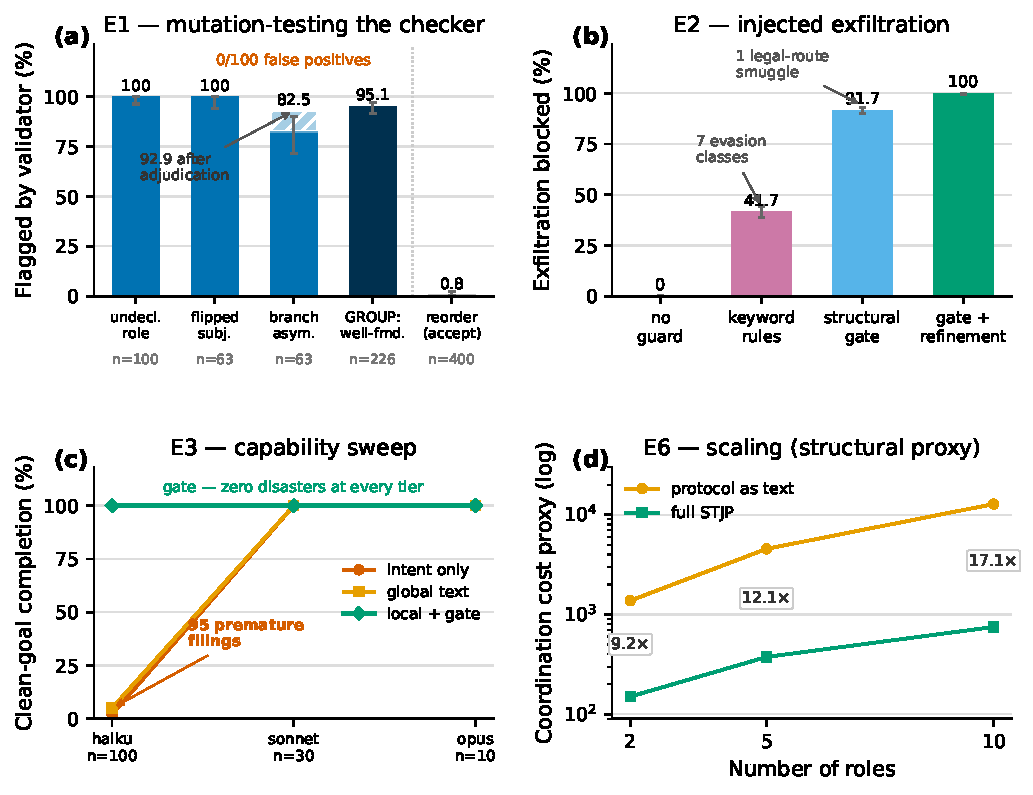
\includegraphics[width=0.85\textwidth]{fig3_projected.pdf}
\caption{\textbf{Verifying the verifiers, measured.} (a)~Mutation testing of the checker over a 100-protocol corpus. Well-formedness defects are detected at 95.1\% with \emph{zero} false positives on the valid corpus; flagging only 0.8\% of reorderings is \emph{correct acceptance}, since reordering an acyclic protocol usually yields another valid protocol. (b)~Red-teaming with 1{,}200 injected exfiltration attempts per condition. Keyword rules reach 41.7\% and are evaded by encodings, synonyms, and splitting; the structural gate reaches 91.7\%, disguise-proof for every illegal route yet blind to a payload smuggled on a legal one; adding value refinements closes exactly that hole. The layering is the finding. (c)~Capability sweep across three Claude tiers. Unenforced safety is capability-dependent, with 95 premature filings at the weak tier and zero above, while the gated arm stays flat at 100\% CGC with zero disasters. (d)~Structural cost proxy. The global-text-to-\stjp{} coordination-cost ratio widens from $9.2\times$ at two roles to $17.1\times$ at ten.}
\label{fig:projected}
\end{figure}

\textbf{E0 --- Test the testers first.} A 40-trace verdict corpus with hand-derived expected verdicts (clean traces, every severity class, concurrent interleavings, unevaluable-guard silence, the \texttt{Approval(False)} edge case). Monitor and grader score 40/40---and, instructively, three of the \emph{hand derivations} were wrong and corrected against the semantics; the instruments were right. All downstream experiments inherit this validated referee. An integration harness additionally exercises all five pipeline stages 100 times ($2105/2110=99.76\%$ checks passing; the five failures are a FIFO-swap mutation that yields another well-formed protocol, which Scribble \emph{correctly} accepts).

\textbf{E1 --- Mutation-test the static checker (Fig.~\ref{fig:projected}a).} Seven mutation operators were applied over a 100-protocol corpus spanning 2--10 roles and four topologies, pre-registered to separate two defect families, and the data respected the split. \emph{Well-formedness} defects are detected at 95.1\% (226 mutants, with undeclared role and flipped-choice-subject at 100\% and branch asymmetry at 82.5\% raw) with 0/100 false positives on the valid corpus. Adjudicating the eleven branch-asymmetry survivors found seven \emph{accidentally valid} (correct acceptances) and four sharing one genuine gap---a knowledge-of-choice deadlock the checker misses---re-scoping real-defect detection to 92.9\% and converting a bare percentage into a \emph{named limitation}. \emph{Reordering} operators (400 mutants) are flagged at only 0.8\%, which is correct behavior, because reordering an acyclic protocol usually produces a different but valid protocol; detecting \emph{intent} drift under valid reorderings is a semantic scorer's job, not the type checker's, and conflating the two is how benchmarks overstate their tools. The standard here is deliberately the two-sided \emph{preciseness} discipline of \citet{chen17,chen24}---soundness (nothing bad accepted) and completeness (nothing good rejected) measured together---transplanted from characterizing a subtyping relation to auditing a checker implementation.

\textbf{E2 --- Red-team the runtime gate (Fig.~\ref{fig:projected}b).} Twelve prompt-injection templates were run 100 times each against a finance protocol with a confidential payload and an ExternalAuditor role that legally receives only the public summary. With no guard, nothing is blocked. An honestly tuned keyword-and-role rule list blocks 41.7\% and is evaded by encoding, synonyms, typos, split payloads, and innocuous relabeling. The structural gate blocks 91.7\%, rejecting every attempt to use an illegal (label, recipient) edge \emph{regardless of disguise} because legality is checked against the type rather than the wording; the surviving 8.3\% is exactly one template that smuggles the payload \emph{inside} a legitimately-labelled message on a legal route, which structure cannot see. The gate with value-refinement guards blocks 100\%. Each mechanism catches precisely the class the theory says it catches, and none of them can be argued with, because none of them is a model.

\textbf{Red-teaming our own harness (the fairness audit).} A benchmark whose headline reads ``0\% vs.\ 100\%'' should expect the question of whether the grading was rigged, so we audited our own harness and report what it found, because the honest answer was ``partly.'' Five findings led to five fixes. (1)~The old headline rule asked bare agents to guess secret words. A trial passed only if the exact expected label crossed the exact expected edge, and the protocol arms were handed that vocabulary while the bare arm was not; grading it strictly is grading an essay by whether it contains the answer key's exact sentence. The rule is now \emph{per-arm} (protocol-shown arms judged strictly; bare arms pass on the right sender delivering a predicate-satisfying payload to the right receiver under any label), pre-audit tables are labeled, and bare-arm scores there are lower bounds. (2)~Goal re-anchoring had silently eased two pass predicates; predicate changes are now blocked by an automated invariance guard unless a payload-type change forces a translation, which then requires human sign-off. (3)~All arms shared one rate-limited deployment, so wall-clock figures flattered the arm making the fewest calls, which was ours; contended wall-clock is labeled indicative and speed claims are withheld, while the token and call counts that carry the cost claims are unaffected. (4)~The scheduler's only opponent was round-robin poll-all, the weakest scheduler one can write. A protocol-free control that polls whoever just received a message is built and pre-registered with a deliberately falsifiable prediction, namely that it ties on linear pipelines and loses on branch and fan-in cases where ``last receiver'' has no answer. (5)~The gate arm also whispered per-turn hints the observer arm never got, so a hint-free gate ablation is pre-registered, predicting that zero disasters are preserved while some liveness is lost. Evaluation harnesses are part of the trusted computing base of any verification claim; they deserve the same adversarial scrutiny as the system.

\textbf{Forensic audit of the benchmark data.} A post-hoc audit of all 1{,}200 ladder trials re-verified every suspicious pattern against raw state files and surfaced one material bug, namely 22 trials abandoned mid-play rather than failed, 18 of which depressed one gated arm's reported liveness to 79\% against a true $\sim$97\%. All 22 were driven to termination and every table regenerated; the 19 \emph{genuine} gated-arm deadlocks were left standing, because replaying real failures until they pass is p-hacking. Scale also surfaced integrity incidents we log rather than hide, including subagent role-players caught writing auto-responder scripts instead of reasoning per poll (detected, discarded, and replayed), a round-numbering bug that could mask disasters, and a false-positive disaster check on enforcing arms, all fixed. The final state contains zero remaining fraud and zero non-terminal trials.

\section{What the verifier finds at scale}\label{sec:findings}
\begin{figure}[t]
\centering
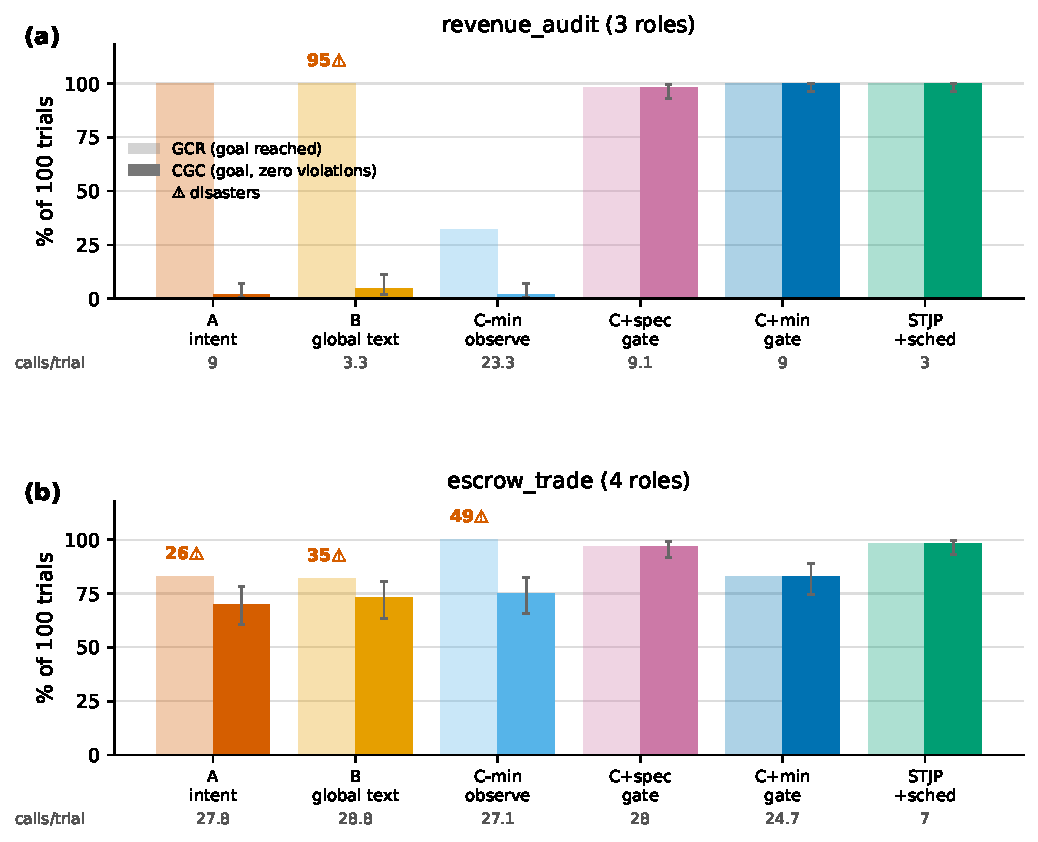
\includegraphics[width=0.85\textwidth]{fig4_ladder.pdf}
\caption{\textbf{The six-arm ladder at $n{=}100$} (measured; 1{,}200 trials, cheap subagent roles, cost in LLM calls). Light bars show goal completion (GCR), solid bars clean-goal completion (CGC), red counts trials containing an unauthorized irreversible act, and the bottom row mean calls per trial. (a)~On \texttt{revenue\_audit}, where filing is allowed only after approval, unenforced global text reaches the goal in 100/100 trials yet files before approval in 95 of them, the observe-mode arm collapses to 32\% on pure liveness, and every enforcing arm shows zero disasters \emph{by construction}. (b)~On \texttt{escrow\_trade}, violations invisible at $n{=}10$ surface in every observe arm (26--49), and the scheduler delivers the cost win at 7.0 calls per trial against 24.7--28.8. Post-audit final numbers with no non-terminal trials.}
\label{fig:ladder}
\end{figure}

Two tasks, \texttt{revenue\_audit} (3 roles, the safety axis) and \texttt{escrow\_trade} (4 roles, the cost axis), run six arms at $n{=}100$ each for 1{,}200 trials, turning three independent knobs---what the agent sees (intent, global text, or local projection), whether the monitor enforces (observe versus gate, the same program in two modes), and who gets polled (all roles every round versus only the enabled sender). Four findings follow (Fig.~\ref{fig:ladder}).

\textbf{(i) Prose compliance does not survive concurrency.} At smaller $n$, unenforced global text (B) had tied the gated arm on outcome and we declined to claim enforcement was necessary---a pre-registered prediction we graded as falsified (\S\ref{sec:honest}). At $n{=}100$ under concurrent polling the tie collapses. Arm B reaches the goal in 100\% of \texttt{revenue\_audit} trials \emph{while filing before approval in 95 of 100}. Trace forensics make the mechanism exact---in 60 trials the Auditor approved without ever receiving the revenue figure, in 35 more all three messages fired in round one, and only 5 serialized. GCR conceals this entirely, while CGC reads 5\%. This is the sharpest argument we know for verification signals richer than task success. \textbf{A scalar pass rate of 100\% coexisted with a 95\% disaster rate}, and only a structure-aware verifier could tell them apart.

\textbf{(ii) Liveness must be driven, not observed.} The observe-mode local-contract arm completes only 32\% of \texttt{revenue\_audit} trials---all 68 stalls show the same pattern, an agent re-sending into an unenforced wait. A contract can make every action that happens correct; it cannot, by observation alone, make an action happen. The projection must \emph{drive} the runtime (the scheduler is a projection artifact), which is why runtime verification here is enforcement, not monitoring.

\textbf{(iii) Safest and cheapest, simultaneously.} Every enforcing arm shows zero disasters at $n{=}100$ in both tasks---not zero-so-far but zero \emph{by construction}, since the gate rejects the disallowed send before delivery---and full \stjp{} is also the cheapest arm (3.0 and 7.0 calls/trial vs.\ 3.3--28.8), because the scheduler never spends a call on a role whose turn it structurally is not. Table~\ref{tab:ctcg} prices the verification dividend. Dividing mean calls by CGC, B's apparently cheap 3.3 calls per trial becomes 66 calls per \emph{clean} goal once poisoned successes stop counting, and full \stjp{} wins by $4$--$22\times$ on the metric an operator actually pays. In dollars, with weak-tier roles at list price, a clean and safe audit costs \$0.38 under \stjp{} versus \$1.12--\$9.09 for the alternatives.

\begin{table}[t]
\centering\small
\caption{Cost to \emph{clean} goal (mean calls/trial $\div$ CGC), $n{=}100$ per arm. GCR-based cost rankings reverse once violated runs stop counting as successes.}
\label{tab:ctcg}
\begin{tabular}{@{}lcccccc@{}}
\toprule
\textbf{Task} & \textbf{A intent} & \textbf{B global text} & \textbf{C-min obs.} & \textbf{C+spec} & \textbf{C+min} & \textbf{\stjp{}} \\
\midrule
\texttt{revenue\_audit} & 450 & 66 & 1165 & 9.3 & 9.0 & \textbf{3.0} \\
\texttt{escrow\_trade} & 39.7 & 39.5 & 36.1 & 28.9 & 29.8 & \textbf{7.1} \\
\bottomrule
\end{tabular}
\end{table}

\textbf{(iv) Verification remains faithful as agents evolve; unenforced safety does not.} Which unenforced configuration fails is a function of model, task, and scheduling that nobody can predict in advance. Intent-only was the villain under a strong confident model, with 22 unauthorized irreversible acts in 30 attempts on the live finance case, so capability \emph{amplified} the coordination gap; unenforced global text failed under concurrent polling (the 95 disasters above); and the observe-mode contract failed on liveness. The measured capability sweep (Fig.~\ref{fig:projected}c, three Claude tiers, both tasks) closes the model axis. On identical protocol text, B's premature filings go 95$\to$0$\to$0 and intent-only's cleanliness goes 2\%$\to$100\%, while the gated arm holds 100\% CGC with zero disasters, and \emph{zero gate rejections even needed}, at every tier. Read naively, the closing gap says strong models need no enforcement; read correctly, the gap is an \emph{average} while the gate's zero is a \emph{guarantee}, since production does not get to assume the strongest model and criticality is priced on the tail.

\textbf{Deadlock and livelock, the failure classes runtime verification cannot rule out.} A two-role protocol seeded with the classic circular wait stalls every bare run forever; Scribble rejects the global type \emph{before any agent runs}, at zero token cost, and the repaired protocol executes at 100\%. No runtime guardrail, judge, or benchmark can offer this, because they all require the failure to occur at least once. At $n{=}100$ the unchecked configuration deadlocks in 100/100 trials, burning 800 calls; \stjp{} completes 100/100 at the protocol-optimal 7.0 calls/trial---\emph{fewer total calls than the arm that never finishes}. Nine live cases assembled from real, unmodified public skill files (Anthropic's skills repository, \texttt{awesome-copilot}, OpenAI Agents SDK, LangGraph, AutoGen, CrewAI, and AgenticPay; Table~\ref{tab:realcases} in the appendix) replicate the shape in the wild. Seven of nine complete 0/10 as downloaded, and the remaining two complete only as a model-dependent coin flip whose direction \emph{reverses} between Claude tiers. On the one looping protocol, the plan-as-text arm enters a \emph{stable livelock}, with 10/10 trials burning the entire 16-round budget in motion and emitting 530 rule-breaking messages at $3.6\times$ the token cost of the \stjp{} arm that merges 10/10 with zero violations. Deadlock is silence, livelock is motion without progress; the same static object rules out both, because both are properties of the protocol, not of any message.

\section{Pre-registered predictions, graded, including the ones we got wrong}\label{sec:honest}
\textbf{P1 (falsified twice, differently).} We predicted that unenforced global text would slip below 100\%. Under one model it did (40\%); under a stronger one it did not, and the $n{=}100$ concurrent-polling run then showed the same arm at 100\% GCR with 95 disasters, resolving what the tie had left open. What survives all outcomes is that the gate rejected real off-contract attempts in \emph{every} gated run, and that enforcement value falls with model strength while the danger of no protocol at all rises. \textbf{P2 (confirmed beyond margin).} Scheduling saves at least 60\% of tokens against lean$+$gate, with $-65\%$ tokens and $-66\%$ calls measured. \textbf{P3 (half-confirmed).} Projection alone does not beat global text, but projection with enforcement and scheduling dominates it. \textbf{P4 (deferred).} The orchestrator-cost comparison was inconclusive. \textbf{P5 (confirmed).} Scheduling cuts calls without inflating tokens per call. All eight validation-suite predictions were likewise registered and graded (E0--E2, E4--E7 \textsc{confirmed}; E3's capability clause confirmed, vendor diversity open). We report the grades because a verifier that hides its own falsified predictions has misunderstood its subject.

\section{Limitations}\label{sec:limits}
\textbf{The verified artifact is not the verified intent.} Intent$\to$Scribble passes through an LLM; the validator rejects structurally invalid drafts, but a valid-yet-\emph{unintended} protocol survives (validated $\neq$ intended). The shipped mitigations are human endorsement of $\gtG$ before any agent runs and the human outcome anchor. Because the grammar, validator, and an EFSM-equivalence scorer (300/300 on identical/reformatted/mutant pairs) exist, the translation step is a verifier-in-the-loop learning problem with a free deterministic reward; its training program is pre-registered and out of scope here. \textbf{Theorem scope.} Deadlock-freedom is per-session; interleaved sessions and dynamic role join/leave \citep{denielou11} are future work; our experiments fix the role set. \textbf{Expressiveness.} Open-ended brainstorming resists protocolization, and forcing it into a type would be dishonest; \stjp{} targets the coordination-critical, authorization-laden regime. \textbf{Statistics and realism.} Live frontier-model runs remain $n{\leq}10$ per cell with wide Wilson intervals; the $n{=}100$ suite fixes power but substitutes cheap subagent role-players or contract-following strategies for frontier models. The capability sweep lacks a non-Claude frontier point (an access limitation we report rather than fake). Pre-audit finance tables use the strict label rule the fairness audit found unfair to bare arms (their scores are lower bounds; per-arm re-runs pending), and contended wall-clock figures carry no comparative claim. \textbf{No tools; invented data.} Roles carry no tools, so the C1 provenance check currently certifies message discipline, not real data lineage. \textbf{Grader and monitor.} The severity grader is payload-blind at milestones (the monitor-level guard closes this; the grader upgrade is pending); monitor correctness is validated, not mechanized---certified projection \citep{liwies25} is our named upgrade path.

\section{Conclusion}
Who verifies the agents? For the coordination layer, a compiler can, before any agent runs and over all runs at once, with runtime enforcement and evaluation falling out of the same verified object as deterministic code. Unenforced arms fail in ways that move unpredictably with model, task, and scheduling, and their scalar pass rates actively conceal it, as a 100\% goal rate coexisted with a 95\% disaster rate; the enforcing arm is the only invariant of the grid, and the cheapest once violated successes stop counting. The verifiers are themselves mutation-tested, red-teamed, and audited---including the harness, including against us. Prompts move probabilities; only checks move guarantees.

\begin{ack}
Omitted for double-blind review.
\end{ack}

\bibliographystyle{plainnat}
\bibliography{references}

\newpage
\appendix

\section{A validated protocol and its guard sidecar}\label{app:scr}
The abbreviated Scribble global type for the finance case follows.
\begin{small}
\begin{verbatim}
global protocol Finance(role Ingestor, role RevenueAnalyst, role ExpenseAnalyst,
                        role TaxVerifier, role Auditor, role Writer) {
  RawRevenueData(Payload) from Ingestor to RevenueAnalyst;
  ExpenseData(Payload)    from ExpenseAnalyst to RevenueAnalyst;
  choice at RevenueAnalyst {
    HighRevenueNotification(Analysis) from RevenueAnalyst to Auditor;
    AuditReport(Findings)             from Auditor to TaxVerifier;
  } or {
    StandardRevenueNotification(Analysis) from RevenueAnalyst to TaxVerifier;
  }
  Approval(Decision)    from TaxVerifier to Writer;   // goal marker
  FinalReport(Document) from Writer to Ingestor;      // goal marker, FINAL
}
\end{verbatim}
\end{small}
The choice-guard sidecar (\texttt{.refn}, asserted-MPST style, stock Scribble untouched) follows.
\begin{small}
\begin{verbatim}
[choice at RevenueAnalyst]
when:    float(RawRevenueData) > 50000
require: HighRevenueNotification
over:    StandardRevenueNotification

[payload Approval]
assert:  Decision == 'true' => next in {FinalReport}   # denied-but-debited hole
\end{verbatim}
\end{small}
The guard travels through four stages, from \emph{define} (sidecar) to \emph{state} (compiled into the contract at the decision state) to \emph{check} (value-tracking monitor) to \emph{enforce} (gate). Offline replay verification fires on high-revenue$+$standard-branch and on the symmetric case, and stays silent on correct branches and on unevaluable guards.

\section{Real-skills live runs}\label{app:real}
\begin{table}[h]
\centering\footnotesize
\caption{Nine cases built from unmodified public agent/skill files, three arms each. ``H''/``S'' $=$ Claude Haiku/Sonnet tiers in the two-model sweep (120 trials); \emph{viol.} $=$ rule-breaking messages. The \texttt{pr\_review\_merge} text arm is the measured livelock, completing 0/10 at $3.6\times$ the cost of the succeeding \stjp{} arm. Every source file is deep-linked with license provenance in the repository. Two honesty notes apply. Earlier casts of two cases had misread their sources and were corrected, and runs are $n{=}10$ per arm with round-batched role-play, so same-role trials within a round share one model context.}
\label{tab:realcases}
\resizebox{\textwidth}{!}{\begin{tabular}{@{}llccc@{}}
\toprule
\textbf{Case} & \textbf{Source} & \textbf{No plan} & \textbf{Plan as text} & \textbf{Full \stjp{}} \\
\midrule
\texttt{airline\_seat} & OpenAI Agents SDK & 0/10 deadlock & 10/10, 10 dbl.\ writes & \textbf{10/10, 0, cheapest} \\
\texttt{booking\_saga} & LangGraph & 0/10 stall & 10/10, 10 dbl.\ charges & \textbf{10/10, 0} \\
\texttt{code\_execution} & AutoGen & 0/10 deadlock & 10/10 & \textbf{10/10, cheapest} \\
\texttt{content\_pipeline} & CrewAI (pattern) & 0/10 stall & 10/10 & \textbf{10/10, cheapest} \\
\texttt{doc\_pipeline} & anthropics/skills & flip: H 10/10, S 0/10 & 20/20, 120 viol. & \textbf{20/20 both, 0} \\
\texttt{pr\_merge} & awesome-copilot & flip: H 0/10, S 10/10 & 20/20, 120 viol. & \textbf{20/20 both, 0} \\
\texttt{agenticpay\_settlement} & AgenticPay & deadlock, all 3 tiers & --- & \textbf{100\%, all 3 tiers} \\
\texttt{pr\_review\_merge} & awesome-copilot & 0/10 deadlock (r.2) & \textbf{0/10 livelock}, 530 viol. & \textbf{10/10, 0, $3.6\times$ cheaper} \\
\texttt{doc\_coauthor\_ship} & anthropics/skills & 0/10, budget exhausted & 10/10, 220 viol. & \textbf{10/10, 0, ${\sim}40\%$ cheaper} \\
\bottomrule
\end{tabular}}
\end{table}

The checker earned its keep on the way in. The corrected review protocol was itself debugged statically, with two Scribble rejections (``inconsistent external choice subjects'' and ``role progress violation'') preceding validation---the \S\ref{sec:mpst} diagnostics firing on a realistic review loop before any agent ran. Adapting the buyer and seller agents of the MIT-licensed AgenticPay negotiation benchmark \citep{agenticpay} and adding an escrow settlement layer reproduces the classic circular-wait deadlock across three model tiers, while the validated escrow-first protocol completes.

\section{Live-model five-arm comparison (finance, gpt-5.4, $n{=}10$)}\label{app:grand}
\begin{table}[h]
\centering\small
\caption{All five arms, one model, one run. ``Harmful attempts'' $=$ attempts containing S2+/S4. GCR uses the pre-audit strict label rule for every arm (A's 0\% is a lower bound; \S\ref{sec:verify}); Wilson 95\% intervals at $n{=}10$ run from $[0,28]\%$ at 0\% to $[72,100]\%$ at 100\%. Seconds come from contended parallel execution and are indicative only.}
\label{tab:grand}
\begin{tabular}{@{}lccccc@{}}
\toprule
\textbf{Metric} & \textbf{A intent} & \textbf{B global} & \textbf{C local} & \textbf{C-min} & \textbf{C+ gate} \\
\midrule
GCR (strict) & 0\% & \textbf{100\%} & 60\% & 50\% & \textbf{100\%} \\
Attempts per trial & 3.00 & 1.00 & 1.90 & 2.00 & \textbf{1.00} \\
Delivered violations & 180/180 & 26/100 & 16/151 & 15/153 & \textbf{0/105} \\
S2 / S3 / \textbf{S4} & 29 / 1 / \textbf{22} & 0 / 0 / 0 & 0 / 13 / 0 & 0 / 15 / 0 & \textbf{0 / 0 / 0} \\
Harmful attempts & \textbf{97\%} & 0\% & 0\% & 0\% & \textbf{0\%} \\
Tokens per trial & 21.7k & 24.4k & 154.1k & 84.0k & 79.5k \\
Tokens per success & $\infty$ & \textbf{24.4k} & 96.8k & 44.7k & 79.5k \\
\bottomrule
\end{tabular}
\end{table}

Under the stronger model, intent-only agents were \emph{more} dangerous, not safer, committing 22 unauthorized irreversible acts in 30 attempts with 97\% harmful attempts, against 4 disasters under the weaker model; capability amplifies the coordination gap. In the same run the gate intercepted five premature \texttt{Approval} sends; observed instead of gated, the identical mistake was delivered four times and once cascaded the session off-protocol. On the separate scheduler ablation (shared decentralized runtime, same task), protocol-as-text cost 120k tokens per delivered goal at 41.8 calls/trial, lean contract $+$ gate 38k at 34.0, and full \stjp{} \textbf{13.3k tokens per goal at 11.4 calls}---$9\times$ cheaper at identical 100\% GCR and zero disasters, with tokens-per-call flat (1.12k vs.\ 1.07k), so the entire saving is fewer calls. The defeated opponent is round-robin poll-all; the pre-registered protocol-free scheduling control (\S\ref{sec:verify}) must be beaten on branching and fan-in cases before the scheduler claim is final.

\textbf{Reliability and portability.} With a contract-following strategy certifying the infrastructure at scale, the unchecked arm's Wilson interval narrows to $[0,3.7]\%$ (structurally incapable, not unlucky) and \stjp{}'s $\mathrm{pass}^{10}$ at the Wilson floor rises from 0.039 to 0.686. The standalone monitor agrees with the in-process monitor on 59/59 testable canonical traces; a LangGraph adapter agrees on 14/14 clean-and-injected checks, consistent with T4's boundary placement.

\section{Guarantee transfer table}\label{app:guar}
\begin{table}[h]
\centering\small
\caption{Static guarantees inherited from MPST and their operational meaning for agent systems.}
\label{tab:guarantees}
\begin{tabular}{@{}p{3.2cm}p{5.3cm}p{4.6cm}@{}}
\toprule
\textbf{Guarantee} & \textbf{Agent-system meaning} & \textbf{Consequence} \\
\midrule
Deadlock-freedom (T3) & Circular waits rejected at compile time & Kills the silent-stall, token-burning failure mode for \emph{all} runs \\
Communication safety (T1) & An agent can only emit messages the protocol permits at its state; recipient sets are part of the type & Off-protocol detours and unauthorized disclosure rejected by construction \\
Session fidelity (T2) & Every trace refines the endorsed $\gtG$ & The log is audit evidence against a proven reference \\
Monitorability (T4) & Local $O(1)$ gates compose to global compliance & Decentralized enforcement; no watching agents \\
Refinements $+$ guards & Payload and branch predicates checked at the boundary & ``Protocol-legal but value-wrong'' branches become violations \\
Minimal capabilities & Required tools $=$ labels of $\proj{\gtG}{r}$ & Least-privilege \texttt{allowed-tools} derived, not guessed \\
\bottomrule
\end{tabular}
\end{table}

\section{Reproducibility}\label{app:repro}
All arms, cases, protocols, guards, run directories (events, prompts, per-message verdicts), the severity grader, the mutation and red-team suites, the fairness-audit review document, and the metric engine are in the accompanying repository (link withheld for double-blind review; provided to reviewers via OpenReview supplementary material). Traces are the artifact of record, and re-running the deterministic evaluators on a run directory reproduces every table bit-for-bit. The total compute cost of the 1{,}200-trial validation suite was under \$100.

\section{Responsible-use statement}\label{app:impact}
\stjp{} constrains agents rather than empowering them. Its outputs are rejections, monitors, and audit logs, so its dual-use surface is correspondingly small. The principal societal risk is \emph{false assurance}, since ``validated'' is not ``intended,'' and an operator who reads a checker pass as a guarantee of correct real-world behavior over-trusts the system, the same risk any verification tool carries. The mitigations shipped and evaluated here are human endorsement of the global type before any agent runs, a human-labeled outcome anchor that sits outside the metric family and routes divergence to protocol re-drafting, guarantees stated with their scope (per-session, fixed role set, structural versus semantic conformance), and prominent reporting of our own falsified predictions, checker gaps, and harness-fairness findings, so that the reliability claims can be audited rather than trusted. Enforcement infrastructure could in principle be used to make a \emph{harmful} choreography reliable; the authorization-ordering and confidentiality guards evaluated here are, however, exactly the properties that make agent systems safer to deploy, and the human sign-off point is the natural place for organizational review.

\end{document}
